\section{Uppgift 1}\label{sec:uppg01}

\subsection{Instruktioner}
\begin{Verbatim}[fontsize=\small]
Skriv ett program där man ska skriva in ett antal heltal. Hur många tal ska den
som kör programmet själv bestämma, dock max 30. Heltalen ska lagras i en array.

Programmet ska sedan beräkna summan av talen, beräkna talens medelvärde
(exakta), ta reda på vilket av talen som är störst och minst. Exempel på hur
utskriften kan se ut (inmatning från tangentbordet = *fetstil*):

Hur många tal vill du mata in (max 30)? *5*
*4*
*5*
*3*
*7*
*6*
Summa: 25
Medelvärde: 5.0
Minsta värde: 3
Största värde: 7
\end{Verbatim}


\subsection{Källkod}
\subsubsection{Lab4Uppg01.java}
\javacode{src/Lab4Uppg01.java}
\caption{Lab4Uppg01.java}
\label{src:uppg01}

\subsubsection{UserInputFilter.java}
\javacode{src/UserInputFilter.java}
\caption{UserInputFilter.java}
\label{src:userinputfilter}

% Screenshots med Bash, terminalfönsterstorlek 90x40
\subsection{Skärmdump}
Se Figur~\ref{fig:uppg01-screenshot} för skärmdump på körning av koden i
Sektion~\ref{src:uppg01} och Sektion~\ref{src:userinputfilter}.

\begin{figure}[htbp]
\centering
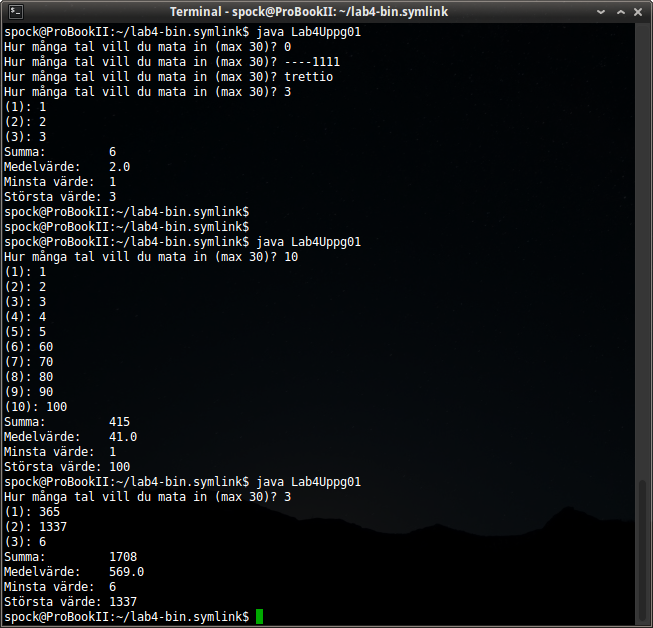
\includegraphics[width=\linewidth]{img/01.png}
\caption{Körning av koden till Uppgift~\ref{sec:uppg01}}
\label{fig:uppg01-screenshot}
\end{figure}

